\documentclass[12pt,a4paper]{article}
\usepackage{amsfonts}
\usepackage{amssymb}
\usepackage{graphicx}
\usepackage{bookmark}
\usepackage{hyperref}
\usepackage{enumitem}
\usepackage{changepage}
\usepackage{float}

\setlength{\parindent}{0em}

\newlist{ConstraintEnum}{enumerate}{1}
\setlist[ConstraintEnum]{label=C-\arabic*:}

\newlist{AssumptionsEnum}{enumerate}{1}
\setlist[AssumptionsEnum]{label=A-\arabic*:}

\newlist{DependenciesEnum}{enumerate}{1}
\setlist[DependenciesEnum]{label=D-\arabic*:}

\newlist{RequirementsEnum}{enumerate}{2}
\setlist[RequirementsEnum,1]{label=R-\arabic*:}
\setlist[RequirementsEnum,2]{label=R-\arabic{RequirementsEnumi}.\arabic*:}

\graphicspath{{CaseDiagrams/}}

\begin{document}

\begin{titlepage}
	\begin{center}
		\begin{figure}[t]
			\centering
			
\includegraphics[width=350px]{Diagrams/logo.PNG}
		\end{figure}
		
		\textsc{\LARGE Requirements Specification for the Bellisimo System}
		
		\textbf{\newline}
		\begin{flushright} \large
		\center  by\newline	
		Martha Mohlala \emph{u10353403}\newline
		\end{flushright}

		\href{https://github.com/Potlake/Bellisimo}{Github} page.\\
		\url{https://github.com/Potlake/Bellisimo}\\

{\large \today}
\end{center}
\end{titlepage}




\tableofcontents
\newpage

\section{Vision and scope}
\subsection{Project background}
Online shopping has grown in popularity over the years. Most people shop online to save time and avoid long queues. There are people who browse through the internet to find where are specials and sales in several stores, and compare the prices amongst the stores. The platform to achieve what mentioned has not readily available to the stores around Hatfield. This becomes a problem when there are specials available and people do not have knowledge of it, and they end up buying items expensively whereas they could have save more on the specials. 
\subsection{Project Vision}
The Bellisimo is a web application that aims at providing an online platform for customers to browse clothing as well as food
catalogues provided by the businesses located in Hatfield. The catalogues include the items and their prices.The systems will provide the latest information regarding the items,sales and specials.

\subsection{Architecture Design of Bellisimo}
The system consists of two subystems that communicate via HTTP using REST framework, and it follows the monolithic architecture where a single unit is deployed.
	\subsubsection{Architectural Patterns}
	The systems follows the Model-View-Controller (MVC) pattern, where the view is the Bellisimo front-end, model is the data model with PostgresSQL database and Controller is Angular2 that communicates with the back-end.
	\subsubsection{Quality Requirements}
	Quality requirements include the following: \newline
	\begin{enumerate}[label=(\alph*)]
	\item Performance
	\item Availability
	\item Maintainability
	\item Scability
	\item Reliability
	\item Accessibility
	\end{enumerate}
	
	\subsubsection{Architectural tactics}
	Load balancing and connection/thread pooling address performance.\\
	Fault detection, recovery and prevention address the availability.

\section{User Module}
\subsection{Scope}
Bellisimo's main function will be to provide an online platform for customers to browse clothing as well as food catalogues provided by the business located in Hatfield.\\
\begin{figure}[!ht]
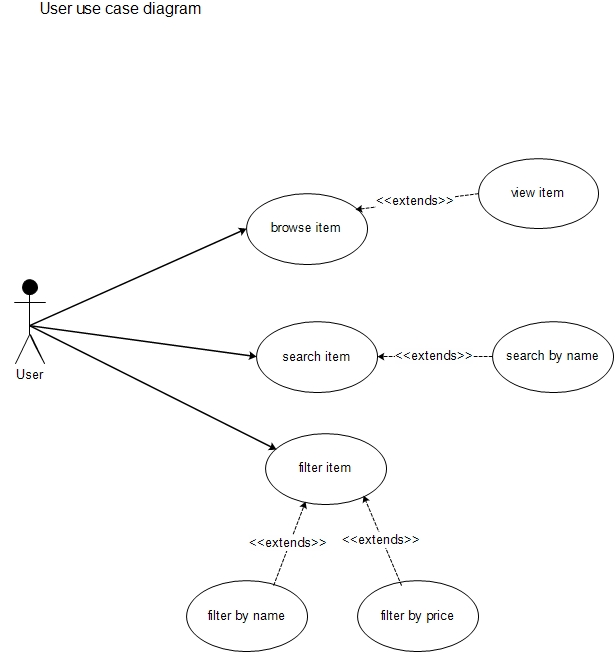
\includegraphics[width=350px]{Diagrams/user_usecase.jpg}
\caption{User use case}
\end{figure}
\textbf{Guest:} No information is stored for the guest user. When accessing the service, the user
assumes the guest role without being logged in. The guest user may use public services and
may register and login.\\
\textbf{User:} When a user is registered, the fields shown in the domain model are stored for the
user, using a unique automatically assigned ID. The user provides all other fields. The
password should be stored in encrypted format. The user may change the value of any of
the fields of his/her own record. The difference
between a user and an admin is the value of the isAdmin field. Only Admin users may
add,remove and update items.\newpage

\textbf{User Class Diagram}
\begin{figure}[!ht]
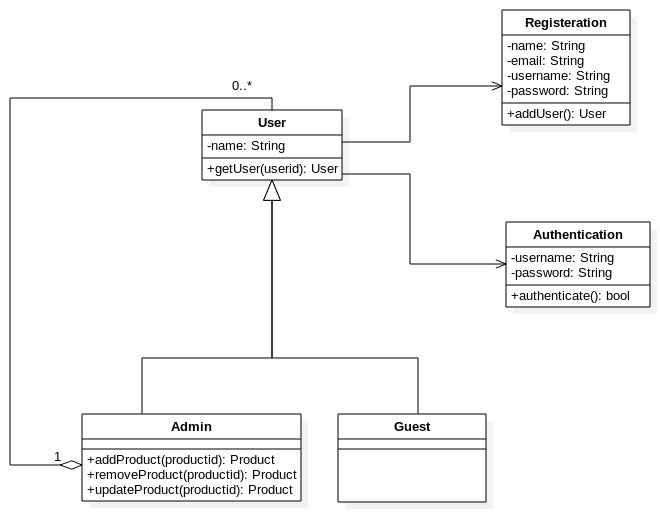
\includegraphics[width=350px]{Diagrams/userclassdiagram.jpg}
\caption{User Class Diagram}
\end{figure}\newpage
The user can wish to register to receive emails about available special. Figure 3 depicts the process of registration.
\begin{figure}[!ht]
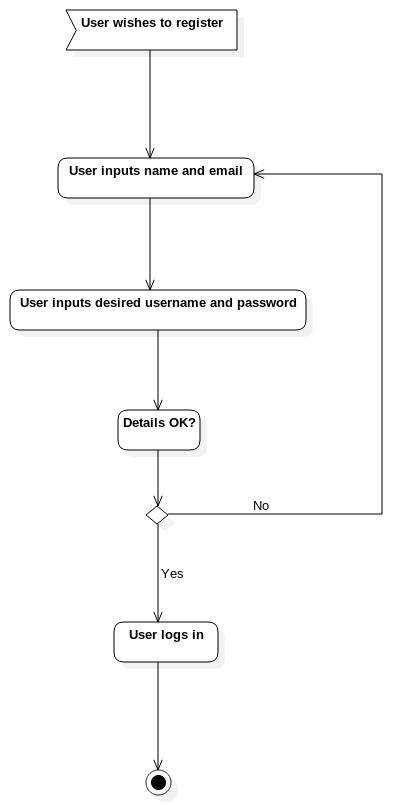
\includegraphics[width=3in]{Diagrams/registerActivityDiagram.jpg}
\caption{Registration Process}
\end{figure} \newpage
\section{Admin Module}
\subsection{Scope}
The admin's main function is to add, delete and update the products. That extends to adding specials. Specials can be added as singular or as a group.\newpage
\begin{figure}[!ht]
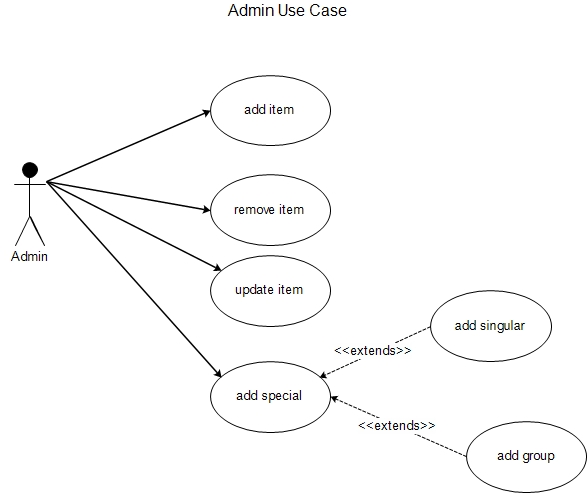
\includegraphics[width=350px]{Diagrams/admin_usecase.jpg}
\caption{Admin Use case}
\end{figure}
The below figure shows the activities perform by the admin.
\begin{figure}[!ht]
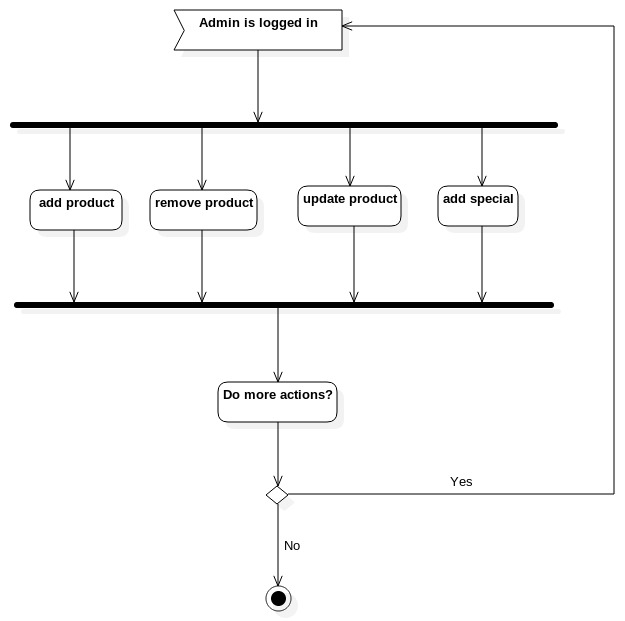
\includegraphics[width=350px]{Diagrams/adminActivityDiagram.jpg}
\caption{Admin activities}
\end{figure}\newpage

\section{Catalogue Module}	
\subsection{Scope}
Catelogues include food items and clothing items from different stores.\newpage
\begin{figure}[!ht]
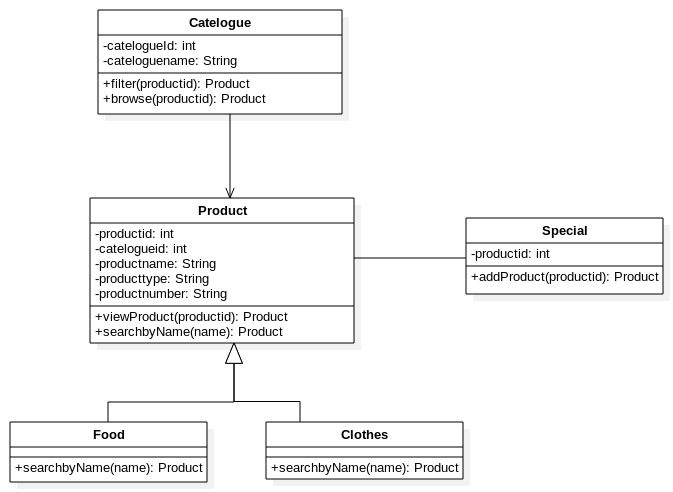
\includegraphics[width=350px]{Diagrams/catelogueclassdiagram.jpg}
\caption{Catelogue Class diagram}
\end{figure}


\section{Technologies}	
\textbf{Html and Bootstrap}: it is used to design the front-end interface.\newline
\textbf{Angular2}: for testing web application. \newline
\textbf{Nodejs}:allows Angular2 and Javascript to run on the server.\newline
\textbf{Spring boot}: implements the back-end of the system to connect to the data model.\newline
\textbf{PostgresSQL}: it used to design and implement database. \newline
\textbf{Apache Maven}: manages the system's build.

\end{document}